\section{Architektur}

Die eigentliche Funktionalität der Bildanalyse und Suche wird in einer Core-Library untergebracht, welche nativ in C++ entwickelt wird.
Die Anzeige der Hilfestellungen für den Spieler soll mithilfe von Unity erfolgen. Unity stellt die Schnittstelle zwischen
dem Spieler und der ganzen Applikation dar und muss sich daher mit der Core-Library austauschen.
Dafür wird eine C/C++-Bibliothek entwickelt, die ein C-Interface zur Core-Library bereitstellt.
Unity lädt diese Bibliothek und wandelt erhaltene native Objekte in Objekte um, welche in Unity verwendet werden können.
Eine Darstellung kann in Abbildung \ref{fig:top-level-architecture} entnommen werden.

\begin{figure}[h!]
    \begin{center}
        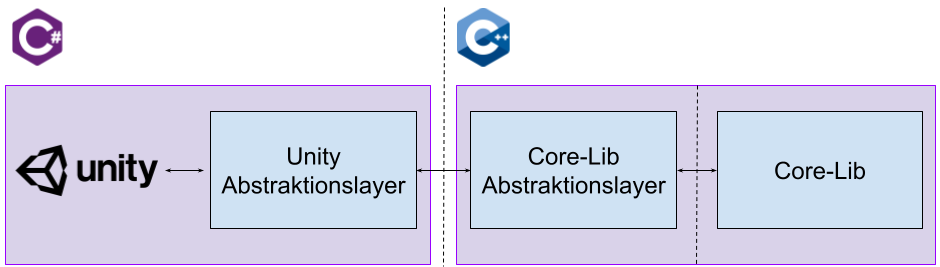
\includegraphics[width=0.8\linewidth]{../common/03_billiard_ai/resources/00_top_level_architecture.png}
    \end{center}
    \caption{Grobarchitektur - Applikationsumgebung}
    \label{fig:top-level-architecture}
\end{figure}

Die Core-Library selbst besteht aus den folgenden Komponenten:
\begin{description}
    \item[billiard\textunderscore capture] Dient als Schnittstelle zur Kamera und stellt die Bilder im OpenCV-Format bereit.
    \item[billiard\textunderscore detection] Erstellt aus dem Spielstand eine interne Repräsentation, welchen den Status beschreibt.
    \item[billiard\textunderscore snooker] Enthält Snooker-spezifische Funktionalität, u.a. die Erkennung der Snooker-Kugeln auf dem Billiardtisch.
    \item[billiard\textunderscore search] Verwendet den aktuellen Status wie auch eine zusätzliche Such-Beschreibung, um einen optimalen
    Stoss zu berechnen.
    \item[billiard\textunderscore physics] Stellt Funktionalität bereit, um physikalische Berechnungen durchzuführen.
\end{description}

Für die Umsetzung der Core-Library wird OpenCV\footnote{Siehe https://opencv.org} 5.4.2 verwendet.
